\chapter*{Schlusswort}
\addcontentsline{toc}{chapter}{Schlusswort}

\section*{Ausblick}
Eigentliches Potenzial von TensorFlow und Keras aufzeigen
\subsection*{Variational Autoencoder}
\subsection*{Generative Adversial Networks}
\subsection*{Recurrent Neural Networks}
\subsection*{Weitere Technische Aspekte}
\subsubsection*{Weitere Kostenfunktionen}
Cross-entropy.
\subsubsection*{Weitere Optimisierungsverfahren}
Adam-Optimizer
Momentum-Optimizer

\subsection*{Frameworks}
TensorFlow 2.0
PyTorch



\section*{Persoenlicher Eindruck}

% ---------------------------------

\begin{appendices}
end{minted}

\chapter{Gradientenverfahren}\label{sec:anhang_gd}
Das Gradientenverfahren ist ein numerisches Verfahren, um Funkionen $f(x_1,
x_2, \ldots, x_n)$ vom Typ $\set{R}^n \to \set{R}$ (wie z.B. die Fehlerfunktion)
zu minimieren.
Dies geschieht, indem ein Startpunkt (Ortsvektor) $\vec{p}_0$ gewählt wird, dessen
Komponenten den Input von $f(\vec{p}_0)$ darstellen.
Nun werden iterativ neue Punkte $\vec{p}_t$ gesucht, welche immer näher beim lokalen Minimun liegen, also Punkte, die den Funktionswert $f(\vec{p}_t)$ immer kleiner werden lassen.
Dies wird durchgeführt, bis der Punkt genügend nahe beim lokalen Minimun ist.
\para{}
Dafür muss ein Vektor $\vec{b}_t$ bestimmt werden, welcher auf den Punkt $\vec{p}_t$ addiert einen neuen Punkt $\vec{p}_{t+1}$ bildet,
bei dem der Funktionswert $f(\vec{p}_{t+1})$ kleiner ist als der von $f(\vec{p}_t)$.
Dies geschieht am effizientesten, wenn $\vec{b}_t$ in die Richtung der stärksten Funktionswertabnahme zeigt.

Hierzu wird man den sogennanten \keyword{Gradient} $\vecf{\nabla}$ verwendet,
für den wiederum partielle Ableitungen benötigt werden.
\para{}
\begin{defbox}{Partielle Ableitungen}\label{ref:partielle_ableitungen}
  Partielle Ableitungen sind eine Erweiterung der ``normalen'' Ableitungen auf
  multidimensionale Funktionen $f(\vec{x}) = f(x_1,\ldots,x_n): \set{R}^n \to \set{R}$.
  Man leitet dabei nur nach einem Argument $x_i$ ab und betrachtet die restlichen Argumente als Konstanten.
  Es gelten die gleichen Ableitungsregeln wie bei der nicht-partiellen Ableitung.
  Die partielle Ableitung einer Funktion $f(x_1,\ldots,x_n)$ bezüglich einer
  Variable $x_i$ in einem Punkt $\vec{a} = \trans{\begin{pmatrix} a_1 & \cdots & a_n \end{pmatrix}}$
  ist analog zur normalen Ableitung folgendermassen definiert:
  \begin{equation*}
    \partderiv{f}{x_i}(\vec{a}) \coloneqq \lim_{h \to 0} \frac{f(a_1,\ldots,a_i + h,\ldots,a_n)-f(a_1,\ldots,a_i,\ldots,a_n)}{h}
  \end{equation*}
  Geometrisch ist dies die Steigung der Tangente an die Kurve der Funktion $f$ im Punkt
  $\vec{a}$. Die Tangente liegt in der Richtung der Achse des Parameters $x_i$,
  nach welchem abgeleitet wurde.
\end{defbox}
\\
\begin{defbox}{Gradient}
  Der Gradient $\vecf{\nabla}$ ist ein Differentialoperator, den man auf eine
  Funktion $f(\vec{x}) = f(x_1,\ldots,x_n): \set{R}^n \to \set{R}$ anwendet kann, welcher ein Skalarfeld auf ein Vektorfeld (das sogennante Gradientenfeld) abbildet.\\
  Um den Gradienten $\vecf{\nabla}f$ der Funktion $f$ zu bilden, fasst man alle partiellen Ableitungen der Funktion $f$, nach jedem
  Argument $x_i$, in einem Vektor zusammen. Meistens bestimmt man den Gradienten
  $\vecf{\nabla} f(\vec{p})$ in einem spezifischen Punkt $\vec{p} =
  \trans{\begin{pmatrix} p_1 & \cdots & p_n \end{pmatrix}}$.
  \begin{equation*}
    \vecf{\nabla}_{\vec{x}} f(\vec{p}) = \ds\partderiv{f}{\vec{x}}(\vec{p}) =
    \begin{pmatrix}
      \ds\partderiv{f}{x_1}(\vec{p}) \\
      \vdots \\
      \ds\partderiv{f}{x_n}(\vec{p}) \\
    \end{pmatrix}
  \end{equation*}

  Geometrisch ist der Gradient $\vecf{\nabla}f(\vec{p})$ einer Funktion $f$ in
  einem Punkt $\vec{p}$ der Vektor, welcher in die Richtung des steilsten
  Anstiegs von $f$ zeigt. Sein Betrag gibt die Stärke des Anstiegs an.
  \para{}
  \begin{center}
    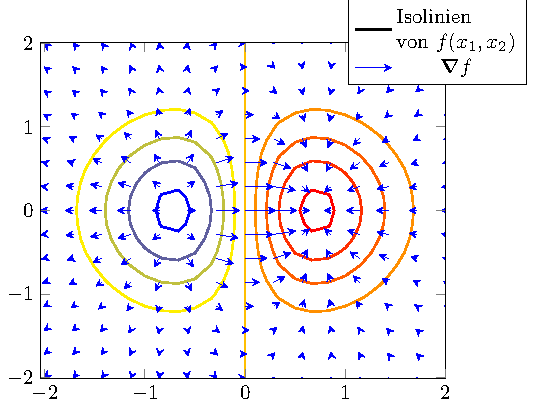
\includegraphics[width=0.7\textwidth]{grad.pdf}
    %\caption{ein Skalarfeld als Konturdiagramm mit zugehörigem Gradientenfeld}
  \end{center}
\end{defbox}
\para{}
Da der Gradient in die Richtung des steilsten Anstiegs zeigt, sollte der Vektor
$\vec{b}_t$ gerade in die entgegengesetze Richtung zeigen. Demnach sollte er in die Richtung des negierten Gradienten der Funktion $f$ im Punkt $\vec{p}_t$ weisen.
Jetzt kann das iterative Annähern an das lokale Minimum folgendermassen beschrieben
werden:
\\
\begin{equation}\label{eq:gradientdescent}
  \vec{p}_{t+1} = \vec{p}_t - \alpha \cdot \vecf{\nabla} \mathit{f}(\vec{p}_t)
\end{equation}
\\
Dabei stellt $\alpha$ einen Proportionalitätsfaktor dar, welcher die
Schrittgrösse beim Abstieg bestimmt.

\ifcp%
\begin{figure}[h!]
  \centering
  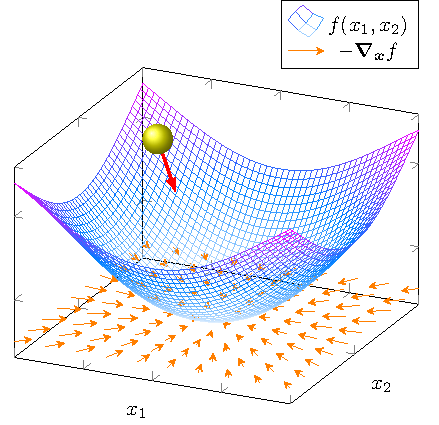
\includegraphics[width=0.5\textwidth]{gd.pdf}
  \caption{Visualisierung des Gradientenabstiegs: Ein Ball rollt das
    Gradientenfeld hinab in das lokale Minimum.}
\end{figure}
\fi%

Während des Gradientenverfahren konvergiert der Punkt $\vec{p}_t$ zu einem
beliebigen \textit{lokalen} Minimum, abhängig davon, wie der Startpunkt
$\vec{p}_0$ gewählt wurde.

\chapter{Herleitung der Rückwärtsprogagierung für KNNs}\label{sec:anhang_bp}
Da ein KNN, wie der Name schon andeutet, vernetzt ist, können die partiellen
Ableitungen einer Schicht anhand seiner Nachbarsschichten berechnet werden.
Dies ist auch der namensgebende Grundgedanke der Rückwärtsprogagierung: Man
beginnt damit die partiellen Ableitung der letzten Schicht zu bestimmen und
berechnet dann retrograd Schicht für Schicht die vorherigen
partiellen Ableitungen, bis zur Inputsschicht. \\
Dies geschieht unter Anwendung der Kettenregel der Ableitungen.
Es ist sinnvoll, für das Aufstellen dieser Gleichungen das Netzwerk als
\keyword{Computational Graph} zu betrachten.
\para{}
\begin{infobox}{Computational Graph}
  Ein Computational Graph ist die Darstellung einer Verkettung von Funktionen als Netzwerk von Operationen.
  Die Knoten im Graph stellen Variablen dar und die Pfade, welche die Knoten
  verbinden, sind die Funktionen, welche die Variablen aufeinander abbilden. Die
  Funktion wird auf die Variable angewendet, von der der Pfad ausgeht. Der Knoten,
  in welchem der Pfad endet, nimmt dann den Funktionswert an. Falls
  mehrere Pfade in einem einzigen Knoten enden, werden die einzelnen Werte der Pfade
  zusammenaddiert, um die Variable zu bilden. In diesem Graphen sind die
  Abhängigkeiten der Variablen voneinander gut ersichtlich. Auf dieser Basis können mithilfe
  der Kettenregel die Ableitungen unkompliziert bestimmt werden.
\end{infobox}
\para{}
\begin{examplebox}{Beispiel: Computational Graph}
  Untenstehend ist ein Beispiel eines Computational
  Graph zusammen mit der Herleitung der partiellen Ableitungen dargestellt.
  \para{}
  \begin{center}
    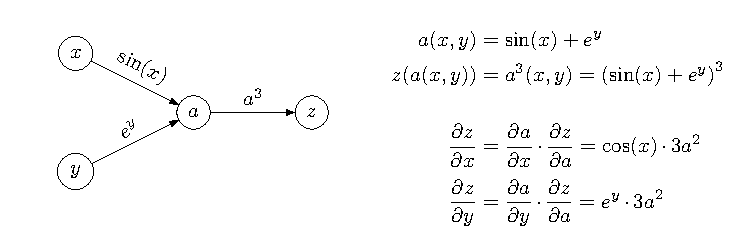
\includegraphics[width=0.8\textwidth]{compgraph.pdf}
    % \caption{Computational Graph einer exemplarischen Verkettung von Funktionen}
  \end{center}
\end{examplebox}
\para{}
\pagebreak
Der erste Schritt der Rückwärtsprogagierung besteht darin, dass die partiellen Ableitungen $\ds\partderiv{C}{z_j^l}$
der Kostenfunktion $C$ bezüglich den gewichteten Summen $z_j^l$ aller Schichten
berechnet werden müssen. Daraus lassen sich dann später die partiellen Ableitungen
bezüglich den Gewichten $\ds\partderiv{C}{w_{j,k}^l}$ und bezüglich den Neigungen
$\ds\partderiv{C}{b_j^l}$ ermitteln.
\para{}
Zur Übersichtlichkeit definiert man einen \keyword{Fehler} $\delta_j^l$ für
jedes $j$-te Neuron in jeder $l$-ten Schicht, welcher die partielle Ableitung bezüglich der
gewichteten Summe dieses Neurons darstellt (siehe Gl. (\ref{eq:BP0}). Ebenfalls definiert man analog einen Fehlervektor
$\vec{\delta}^l$, welcher alle Fehler $\delta_j^l$ einer Schicht $l$
zusammenfasst (siehe Gl. (\ref{eq:BP0a})). Nun heisst es, diesen Wert für jedes Neuron jeder Schicht zu
berechnen.
\\
\begin{gather}
  \tag{BP0}\label{eq:BP0} \delta_j^l \coloneqq \partderiv{C}{z_j^l} \\
  \tag{BP0a}\label{eq:BP0a} \vec{\delta}^l \coloneqq \trans{\begin{pmatrix} \ds\partderiv{C}{z_1^l} & \ds\partderiv{C}{z_2^l} & \cdots & \ds\partderiv{C}{z_{|l|}^l} \end{pmatrix}}
\end{gather}
\\
Da die Kostenfunktion unmittelbar auf die letzte Schicht $L$ angewendet wird, beginnt
dort auch die Berechnung des Fehlers $\vec{\delta}^L$.
Nun wird ein Computational Graph aufgestellt, um die partiellen Ableitungen zu bestimmen.
\para{}
\begin{figure}[h!]
  \centering
  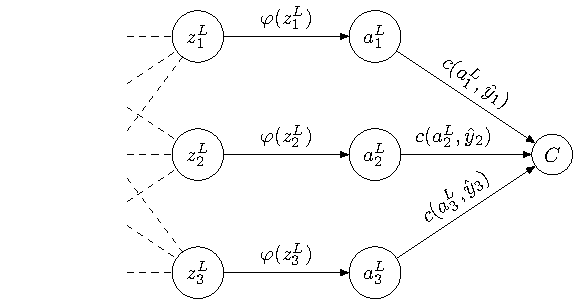
\includegraphics[width=0.7\textwidth]{del_l.pdf}
  \caption{Computational Graph zur Berechnung von $\vec{\delta}^L$}
  \label{fig:cg_L}
\end{figure}
\para{}
Aus dem Computational Graph der Abbildung (\ref{fig:cg_L}) kann entnommen werden, dass die Kosten $C$ eine Funktion
in Abhängigkeit von den letzten Aktivierungen $a_j^L$ ist. Diese ist wiederum
eine Funktion in Abhängigkeit von der jeweiligen gewichteten Summe $z_j^L$.
Somit kann mithilfe der Kettenregel die Beziehung (\ref{eq:BPh1})
aufstellt werden.
\\
\begin{equation}\label{eq:BPh1}
  \delta_j^L = \partderiv{C}{z_j^L} = \partderiv{C}{a_j^L} \cdot \partderiv{a_j^L}{z_j^L}
\end{equation}
\\
Da $a_j^L$ durch die Anwendung der Aktivierungsfunktion $\varphi$ auf $z_j^L$
gebildet wird, ist $\ds\partderiv{a_j^L}{z_j^L}$ die Ableitung der Aktivierungsfunktion
$\varphi'(z_j^L)$. Auf diese Weise lässt sich die erste (\ref{eq:BP1}) von vier
wichtigen Gleichungen für die Rückwärtsprogagierung herleiten.
\\
\begin{equation}\tag{BP1}\label{eq:BP1}
  \delta_j^L = \partderiv{C}{a_j^L} \cdot \varphi'(z_j^L)
\end{equation}
\\
Um diese Ausdrücke wieder in Matrixschreibweise zu realisieren,
welche die ganze Schicht $L$ zusammenfasst, muss eine
neue Operation eingeführt werden: das Hadamard-Produkt.

\begin{defbox}{Hadamard-Produkt}
  Das Hadamard-Produkt (auch elementweises Produkt) ist eine spezielle Multiplikation zweier gleichgrosser Matrizen
  $\mat{A} \in \set{R}^{m \times n}$ und $\mat{B} \in \set{R}^{m \times n}$.
  Die resultierende Matrix ergibt sich aus der elementweisen Multiplikation der Ausgangsmatrizen.

  \begin{minipage}{0.5\textwidth}
    \begin{equation*}
      \mat{A} \odot \mat{B} =
      \begin{pmatrix}
        \matelem{A}_{1,1} \matelem{B}_{1,1} & \cdots & \matelem{A}_{1,n} \matelem{B}_{1,n} \\[0.3em]
        \vdots & \ddots & \vdots \\[0.3em]
        \matelem{A}_{m,1} \matelem{B}_{m,1} & \cdots & \matelem{A}_{m,n} \matelem{B}_{m,n} \\[0.3em]
      \end{pmatrix}
      \in \set{R}^{m \times n}
    \end{equation*}
  \end{minipage}
  %
  \begin{minipage}{0.5\textwidth}
    \begin{equation*}
      \vec{v} \odot \vec{w} =
      \begin{pmatrix}
        v_1 w_1 \\
        \vdots \\
        v_n w_n
      \end{pmatrix}
    \end{equation*}

  \end{minipage}
\end{defbox}
\para{}

Mit $\vecf{\varphi}'$ als die vektorisierte Ableitung der Aktivierungsfunktion,
kann der Fehlervektor der letzten Schicht nach Gleichung (\ref{eq:BPh0})
berechnen werden.

\begin{equation}\label{eq:BPh0}
  \vec{\delta}^L = \trans{\begin{pmatrix} \ds\partderiv{C}{a_1^L} & \ds\partderiv{C}{a_2^L} & \cdots & \ds\partderiv{C}{a_{|L|}^L}\end{pmatrix}} \odot \vecf{\varphi}'[\vec{z}^L]
\end{equation}

Dabei ist der erste Operand des Hadamard-Produkts nichts anderes als
der Gradient $\vecf{\nabla}_{\vec{a}^L} C$ der Kostenfunktion $C$ bezüglich dem Aktivierungsvektor
$\vec{a}^L$ der letzten Schicht. Dieser Gradient kann ermittelt werden, indem die
vektorisierte Ableitungsfunktion für die gewählte Kostenfunktion gebildet wird. Würde die
Mittlere quadratischen Abweichung $C = \frac{1}{2|L|}(\vec{\hat{y}} -
\vec{a}^L)^2$ als Kostenfunktion gewählt werden, ergibbt sich
$\vecf{\nabla}_{\vec{a}^L} C = (\vec{a}^L - \vec{\hat{y}}) \cdot \frac{1}{|L|}$.
\para{}
Daraus folgt die kompakte Matrix-Version (\ref{eq:BP1a}) der Gleichung
(\ref{eq:BP1}), welche den Fehlervektor für die letzte Schicht berechnet.
\\
\begin{equation}\tag{BP1a}\label{eq:BP1a}
  \vec{\delta}^L = \vecf{\nabla}_{\vec{a}^L}C \odot \vecf{\varphi}'(\vec{z}^L)
\end{equation}
\\
Nun soll eine rekursive Berechnungsmethode des Fehlers $\delta_j^{l-1}$
der vorherigen Schicht anhand des Fehlers $\delta_j^l$ der jetzigen Schicht
erarbeiten werden. Zu diesem Zweck ist wiederum ein Computational Graph aufzustellen
(siehe Abb. (\ref{fig:cg_L-1})).
\para{}
\begin{figure}[h!]
  \centering
  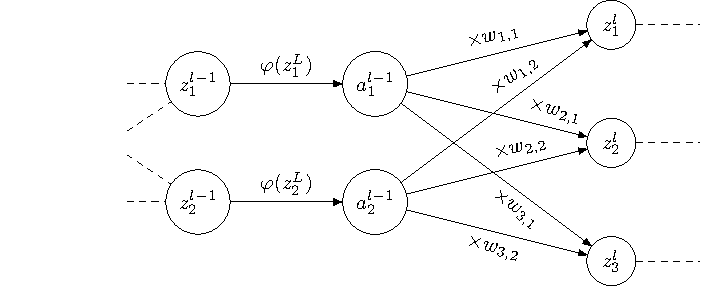
\includegraphics[width=0.7\textwidth]{del_l-1.pdf}
  \caption{Computational Graph zur Berechnung von $\delta_j^{l-1}$}
  \label{fig:cg_L-1}
\end{figure}
\para{}
Es gilt erneut die Gleichung (\ref{eq:BPh1}) für die Berechnung des Fehlers $\delta_j^{l-1}$.
\\
\begin{equation}\tag{\ref{eq:BPh1}}
  \delta_j^{l-1} = \partderiv{C}{z_j^{l-1}} = \partderiv{a_j^{l-1}}{z_j^{l-1}} \cdot \partderiv{C}{a_j^{l-1}}
\end{equation}
\\
Der erste Faktor entspricht der Ableitung $\varphi'(z_j^{l-1})$ der Aktiverungsfunktion.
Beim Übergang einer Schicht ($l-1$) zur Schicht $l$ beinflusst eine Aktivierung
$a_j^{l-1}$ alle gewichteten Summen $z_k^l$. Mit der Kettenregel folgt daher,
dass die partielle Ableitung $\ds\partderiv{C}{a_j^{l-1}}$ die Summe aller
$\ds\partderiv{C}{z_k^l} \cdot \ds\partderiv{z_k^l}{a_j^{l-1}}$ sein muss.
Daraus ergibt sich Gleichung (\ref{eq:BPh2}).
\\
\begin{equation}\label{eq:BPh2}
  \delta_j^{l-1} = \varphi'(z_j^{l-1}) \cdot \sum_{k=1}^{|l|} \left( \partderiv{C}{z_k^l} \cdot \partderiv{z_k^l}{a_j^{l-1}} \right)
\end{equation}
\\
Um die gewichtete Summe $z_k^l$ zu bilden, wird
Aktivierung $a_j^{l-1}$ der vorherigen Schicht mit den entsprechenden Gewichten
$w_{k,j}^{l-1}$ multipliziert.
Dadurch entspricht diese partielle Ableitung $\ds\partderiv{z_k^l}{a_j^{l-1}}$ gerade dem
Gewicht selbst. Desweiteren ist $\ds\partderiv{C}{z_k^l}$ per Definition der
Fehler $\delta_k^l$. Mit dieser Erkenntnis lässt sich die zweite essentielle
Gleichung (\ref{eq:BP2}) für die Rückwärtsprogagierung aufstellen.
\\
\begin{equation}\tag{BP2}\label{eq:BP2}
  \delta_j^{l-1} = \varphi'(z_j^{l-1}) \cdot \sum_{k=1}^{|l|} \left( \delta_k^l \cdot w_{k,j}^{l-1} \right)
\end{equation}
\\
Auch diese Gleichung soll in der Matrixschreibweise dargestellt werden. Zu
diesem Zweck wird der Erweiterungen auf alle gewichteten Summen begonnen:
\\
\begin{equation*}
  \vec{\delta}^{l-1} = \vecf{\varphi}'[\vec{z}^{l-1}] \odot \trans{\begin{pmatrix} \ds\sum_{k=1}^{|l|} w_{k,1}^{l-1} \cdot \delta_k^l & \cdots & \ds\sum_{k=1}^{|l|} w_{k,|l-1|}^{l-1} \cdot \delta_k^l \end{pmatrix}}
\end{equation*}
\\
Der zweite Operant des Hadamard-Produkts ist hierbei gerade das Produkt der
Matrixmultiplikation zwischen
der transponierten Gewichtsmatrix $\trans{(\mat{W}^{l-1})}$ der Schicht ($l-1$)
und dem Fehlervektor $\vec{\delta}^l$ der Schicht $l$.

\begin{gather*}
  \trans{\begin{pmatrix} \ds\sum_{k=1}^{|l|} w_{k,1}^{l-1} \cdot \delta_k^l & \cdots & \ds\sum_{k=1}^{|l|} w_{k,|l-1|} \cdot \delta_k^l \end{pmatrix}} =
  \begin{pmatrix}
    w_{1,1}^{l-1} & w_{2,1}^{l-1} & \cdots & w_{|l|,1}^{l-1} \\
    w_{1,2}^{l-1} & w_{2,2}^{l-1} & \cdots & w_{|l|,2}^{l-1} \\
    \vdots & \vdots & \ddots & \vdots \\
    w_{1,|l-1|}^{l-1} & w_{2,|l-1|}^{l-1} & \cdots & w_{|l|,|l-1|}^{l-1}
  \end{pmatrix}
  \trans{\begin{pmatrix} \delta_1^l & \cdots & \delta_{|l|}^l \end{pmatrix}} \\=
  \trans{\begin{pmatrix}
      w_{1,1}^{l-1} & w_{1,2}^{l-1} & \cdots & w_{1,|l-1|}^{l-1} \\
      w_{2,1}^{l-1} & w_{2,2}^{l-1} & \cdots & w_{2,|l-1|}^{l-1} \\
      \vdots & \vdots & \ddots & \vdots \\
      w_{|l|,1}^{l-1} & w_{|l|,2}^{l-1} & \cdots & w_{|l|,|l-1|}^{l-1}
    \end{pmatrix}}
  \vec{\delta}^l = \trans{(\mat{W}^{l-1})} \vec{\delta}^l
\end{gather*}
\para{}
Damit wurde die die rekursive Fehlerdefinition in Matrixschreibweise
abbgebildet. Und wir erhalten die kompakte Version (\ref{eq:BP2a}) der zweiten wichtigen Formel (\ref{eq:BP2}).
\\
\begin{equation}\tag{BP2a}\label{eq:BP2a}
  \vec{\delta}^{l-1} = (\trans{(\mat{W}^{l-1})} \vec{\delta}^l) \odot \vecf{\varphi}'[\vec{z}^{l-1}]
\end{equation}
\\
In einem letzten Schritt sind nun noch die noch Formeln herzuleiten, mit welchen
anhand des Fehlers $\delta_j^l$ die partiellen Ableitungen der Gewichte und
der Neigungen berechnen werden können.
\para{}
Eine Neigung $b_j^l$ ist Funktionsbestandteil der entsprechenden gewichteten
Summe $z_j^{l+1}$. Somit gilt für die Neigung Formel (\ref{eq:BPh3}).
\\
\begin{equation}\label{eq:BPh3}
  \partderiv{C}{b_j^l} = \partderiv{C}{z_j^{l+1}} \cdot \partderiv{z_j^{l+1}}{b_k^l}
\end{equation}
\\
Der erste Term ist hierbei per Definition der Fehler $\delta_j^{l+1}$ und der
zweite Term lässt sich auf 1 kürzen, da die Summe $z_k^{l+1}$ nur aus
$b_k^l$ besteht und aus Summanden, welche für die partielle Ableitung als konstant gelten.
Somit entspricht die Ableitung der Neigung gerade dem Fehler, womit die
dritte (\ref{eq:BP3}) von vier essentiellen Gleichungen ermittelt wurde.
\\
\begin{equation}\tag{BP3}\label{eq:BP3}
  \partderiv{C}{b_j^l} = \delta_j^{l+1}
\end{equation}
\\
Somit entspricht der Kostengradient bezüglich der Neigung dem Fehlervektor.
\\
\begin{equation}\tag{BP3a}\label{eq:BP3a}
  \vecf{\nabla}_{\vec{b^l}} C =  \vec{\delta}^{l+1}
\end{equation}
\\
Ein Gewicht $w_{j,k}^l$ ist ebenfalls ein Funktionsbestandteil der assozierten
gewichteten Summe $z_j^{l+1}$. Dadurch gilt für die partiellen Ableitungen der
Kosten nach dem Gewicht die Gleichung (\ref{eq:BPh4}).
\\
\begin{equation}\label{eq:BPh4}
  \partderiv{C}{w_{j,k}^l} = \partderiv{C}{z_j^{l+1}} \cdot \partderiv{z_j^{l+1}}{w_{j,k}^l}
\end{equation}
\\
Dabei lässt sich der erste Teil der Gleichung entspricht wieder dem Fehler $\delta_j^{l+1}$.
Die zweite partielle Ableitung ist gerade die Aktivierung $a_k^l$, da sich die
gewichtete Summe aus der Multiplikation des Gewichtes mit der Aktivierung ergibt.
Auf diese Weise ensteht die letzte der vier essentiellen Gleichungen (\ref{eq:BP4}).
\begin{equation}\tag{BP4}\label{eq:BP4}
  \partderiv{C}{w_{j,k}^l} = \delta_j^{l+1} \cdot a_k^l
\end{equation}
\\
Die Matrix-Version lässt sich als Gleichung (\ref{eq:BP4a}) ausdrücken.
\begin{equation}\tag{BP4a}\label{eq:BP4a}
  \vecf{\nabla}_{\mat{W}^l} C = \vec{\delta}^{l+1} \trans{(\vec{a^l})}
\end{equation}

\begin{graybox}{Zusammenfassung Rückwärtsprogagierung}
  \begin{enumerate}
    \setcounter{enumi}{-1}
  \item{Vorwärtspropagierung durchführen und dabei alle Zwischenwerte beibehalten.}
    \item{Berechnung des Fehlers $\vec{\delta}^L$ der letzten Schicht, anhand
        der Formel:
      \begin{equation}\tag{BP1a}
        \vec{\delta}^L = \vecf{\nabla}_{\vec{a}^L}C \odot \vecf{\varphi}'(\vec{z}^L)
      \end{equation}
      }
      \item{Rekursive Berechnung des Fehlers $\vec{\delta}^{l-1}$ der jeweils
          vorherigen Schicht, anhand der Formel:
          \begin{equation}\tag{BP2a}
            \vec{\delta}^{l-1} = (\trans{(\mat{W}^{l-1})} \vec{\delta}^l) \odot \vecf{\varphi}'[\vec{z}^{l-1}]
          \end{equation}
        }
      \item{Berechnung des Kostengradienten bezüglich der Neigungen, anhand der Formel:
          \begin{equation}\tag{BP3a}
            \vecf{\nabla}_{\vec{b^l}} C =  \vec{\delta}^{l+1}
          \end{equation}
        }
      \item{Berechnung des Kostengradienten bezüglich den Gewichten anhand der Formel:
          \begin{equation}\tag{BP4a}
            \vecf{\nabla}_{\mat{W}^l} C = \vec{\delta}^{l+1} \trans{(\vec{a^l})}
          \end{equation}
        }
      \item{Gewichte und Neigung mit SGD aktualisieren}
  \end{enumerate}
\end{graybox}

\para{}
\cite{Nielsen}
\cite{rojas}

\chapter{Ausfuehrungen zu TensorFlow}\label{sec:anhang_tf}
\section*{Devices}
Die Kernstücke des Masters sind die verschiedenen \keyword{Devices}, auf
welchen die Berechnungen ausgeführt werden. Ein Device ist jedliche Art von
Computerprozessor, auf welchem die Graphen ausführt werden können.
Zu diesen Prozessoren gehören die CPU (Hauptprozessor) und die GPU (Grafikprozessor).
\footnote{
  Die normale TensorFlow Version ist nicht in der Lage die GPU zu verwenden. Um
  sie verfügbar zu machen, muss man die GPU Version installieren. Wir werden im folgenden
  von der GPU-Version ausgehen, da sie erhebliche Performance Vorteile gewährt.
}
\para{}

Der Master analysiert die verfügbaren Devices und bewertete sie, bezüglich
ihren Fähigkeiten. Anhand dieser Bewertung entscheidet der Master dann, auf
welchem Device die Berechnugen ausgefürt werden.
\footnote{
  Es ist möglich die Graphen auf mehreren Devices gleichzeitig auszuführen und
  so noch schneller die Modelle zu trainieren. Dies ist jedoch erst für sehr
  aufwendige Projekte nötig und erfordert ein fortgeschritteneres Versteantniss.
}
Insofern GPUs zur Verfügung stehen, wählt TF grundsätzlich immer diese, da
sie Tensoroperationen deutlich schneller als CPUs verarbeiten können.

\section*{Performance und Hardwarebeschleunigung}
Nun möchten wir die Gründe für die beachtliche Performance von TF erschliessen.
Der erste wichtiger Faktor dabei ist, dass der Master hauptsächlich in C++
geschrieben ist. C++ ist eine Programmiersprache die sehr nahe am Maschinen-Code
(engl.: low-level) ist. Somit ist der Code sehr hardwarenah und kann so
schneller ausgeführt werden. Der Nachteil besteht dafür darin, dass die Programmiersprache
ziemlich verbos ist. Das bedeutet man braucht viel Code um eine relativ einfach Idee
auszudrücken. Deshalb wurde der Client von TF in Python geschrieben, was
Abhilfe verschafft und so ein relativ einfaches und unverboses Entwickeln ermöglicht.
\para{}
Der andere wichtige Aspekt für die Performance ist wohl die sogennante
\keyword{Hardwarebeschleuniging} (engl. Hardware Acceleration), von welcher TF
gebrauch macht. \\
Hardwarebeschleunigung bezeichnet eine Sammlung an Methoden,
bei welchen man spezialisierte Hardware verwendet um rechenintensive Aufgaben
schneller auszuführen. Die Architektur einer CPU ist zwar so ausgelegt, dass
sie beliebige Aufgaben ausführen kann, jedoch meistens nicht besonders
effizient. Deshalb wurden einerseits neue externe Hardwarebausteine, wie die
GPU, welche sich für Grafikberechnungen besonders eignet, entwickelt.
Andererseits wurde auch die interne Architektur der CPU so angepasst, dass sie
auch spezielisierte Aufgaben besser meistert.
\para{}
Der Grossteil der Hardwarebeschleunigung wird durch die
\keyword{Parallelisierung} von Operationen erreicht. Dabei spaltet man eine
rechenintensive Aufgabe in viele Teilaufgaben auf, welche gleichzeitig in
gleicher Weise ausgeführt werden. Voraussetzung dafür ist, dass die
Teilaufgaben unabhängig voneinander bearbeitet werden können. \\
Ein typisches Beispiel für die Paralleliserbarkeit von Operationen ist die
Matrixmultiplikation. Möchte man eine Matrix $\mat{A} \in \set{R}^{n \times m}$ mit
einer zweiten Matrix $\mat{B} \in \set{R}^{m \times p}$ multiplizieren, muss man
praktisch $m$-mal die gleichen Schritte ausführen: Man berechnet jeweils das
Skalarprodukt zwischen der $i$-ten Zeile von $\mat{A}$ und der $i$-ten Spalte
von $\mat{B}$. Alle diese Skalarprodukte haben keinen Einfluss aufeindander und
können so unabhänigig mit der gleichen Prozedur berchnet werden.
\para{}
Allgemein eignen sich Tensoroperatiön für Parallelisierung und damit zur Hardwarebeschleunigung.
Nun ist auch ersichtlich, weshalb TensorFlow als Hauptdatentyp Tensoren
verwendet; damit es gebrauch von der Hardwarebeschleunigung machen kann. wir fast alle Gleichungen des Maschinellen

\subsection*{CPU-Beschleunigung}
Die Hardwarebeschleunigung der CPU ist für TensorFlow nur von geringfügiger
Relevanz, da TF sich vorallem für GPU-Hardwarebeschleunigung eignet
und dafür optimiert ist. Ausserdem ist es praktisch unmöglich die gleiche
Performance von TF mit einer CPU zu erreichen, welche mit einer GPU möglich ist.
\para{}
Hauptsächlich parallelisiert TensorFlow mithilfe von der \keyword{SIMD}. SIMD
ist ein Prinzip zur Paralleliserung einer Insturktion für mehrere
Dateneinheiten und steht deshalb für ``Single Instruction, Multiple Data''.
SIMD umfasst einerseits die spezifische CPU-Architektur und den dazugehörigen
Befehlssatz, um die Operatiön zu parallelisieren.
Es gibt verschiedene

SSE4.1, SSE4.2, AVX, AVX2, FMA

\subsection*{GPU-Beschleunigung durch cuDNN und CUDA}
cuDNN ist die NVIDIA CUDA Deep Neural Network library. Sie ist eine
GPU-beschleunigte Bibliothek für deep neural networks. Sie stellt
implementation für standard routines wie Vorwärts- und Rückwärtspropagierung bereit.

\subsection*{CUDA}
\subsection*{cuDNN}


\subsubsection*{Automatische Gradientenberechnung}
Als wir die Rückwärtsprogagierung hergeleitet haben, haben wir mithilfe von
Computational Graphs die Kettenregel angewandt um die partiellen Ableitungen zu
bilden. Genau das gleiche macht TF, jedoch automatisiert. Aus diesem Grund ist
TF auch datenstromorient.


% Many optimization algorithms including common ml training algorithms like SGD
% compute the gradient of a cost function with respect to a set of inputs.
% Therefor TF has a built-in support for automatic gradient computation.
% It extends the TF Graph using following procedure:
% If TF needs to compute the gradient of a tensor $C$ with respect to some tensor
% $I$ it first finds the path in the computational graph from $I$ to $C$. It then
% backtracks from $C$ to $I$ and for each operation on the backward path it adds a
% node to the graph composing the partial gradients using the chain rule. The
% newely added node computes the gradient function for the corresponding operation
% in the forward path.
% Code: [db,dW,dx] = tf.gradients(C, [b,W,x])

\chapter{Programmcode}

\begin{minted}[frame=lines,framesep=2mm,baselinestretch=1.2,bgcolor=lightgray,fontsize=\footnotesize,linenos]{python}
import numpy as np
import matplotlib.pyplot as plt

import tensorflow as tf

# MNIST-Datensatz laden
(x_train, _), (x_test, _) = tf.keras.datasets.mnist.load_data()

# Daten formatieren
x_train = x_train.astype('float32') / 255.0
x_test = np.reshape(x_test, (len(x_test), 28, 28, 1))
x_test = x_test.astype('float32') / 255.0
x_train = np.reshape(x_train, (len(x_train), 28, 28, 1))

# verrauschte Bilder (Input) generieren
noise_factor = 0.5
x_train_noisy = x_train + noise_factor * np.random.normal(loc=0.0, scale=1.0, size=x_train.shape)
x_test_noisy = x_test + noise_factor * np.random.normal(loc=0.0, scale=1.0, size=x_test.shape)
x_train_noisy = np.clip(x_train_noisy, 0.0, 1.0)
x_test_noisy = np.clip(x_test_noisy, 0.0, 1.0)

# Modell definieren
input_data = tf.keras.Input(shape=(28, 28, 1))
econv0 = tf.keras.layers.Conv2D(filters=32, kernel_size=(3, 3), strides=(1, 1), padding='same', activation='relu', kernel_initializer='glorot_normal')(input_data)
emaxpool0 = tf.keras.layers.MaxPooling2D(pool_size=(2, 2), strides=None, padding='same')(econv0)
econv1 = tf.keras.layers.Conv2D(filters=32, kernel_size=(3, 3), strides=(1, 1), padding='same', activation='relu', kernel_initializer='glorot_normal')(emaxpool0)
emaxpool1 = tf.keras.layers.MaxPooling2D(pool_size=(2, 2), strides=None, padding='same')(econv1)
encoded =  emaxpool1
dconv0 = tf.keras.layers.Conv2D(filters=32, kernel_size=(3, 3), strides=(1, 1), padding='same', activation='relu', kernel_initializer='glorot_normal')(encoded)
dupsample0 = tf.keras.layers.UpSampling2D(size=(2, 2), interpolation='nearest')(dconv0)
dconv1 = tf.keras.layers.Conv2D(filters=32, kernel_size=(3, 3), strides=(1, 1), padding='same', activation='relu', kernel_initializer='glorot_normal')(dupsample0)
dupsample1 = tf.keras.layers.UpSampling2D(size=(2, 2), interpolation='nearest')(dconv1)
dconv2 = tf.keras.layers.Conv2D(filters=1, kernel_size=(3, 3), strides=(1, 1), padding='same', activation='sigmoid', kernel_initializer='glorot_normal')(dupsample1)
decoded = dconv2

# Modell kompilieren
autoencoder = tf.keras.Model(input_data, decoded)
autoencoder.compile(optimizer='sgd', loss='mean_squared_error')

print(autoencoder.summary())

# Modell trainieren und als Modelldatei speichern
autoencoder.fit(x=x_train_noisy, y=x_train, batch_size=128, epochs=100, shuffle=True, validation_data=(x_test_noisy, x_test), callbacks=[tf.keras.callbacks.TensorBoard(log_dir='/tmp/denoiser', histogram_freq=0, write_graph=False)])
autoencoder.save('denoiser.model')

# Vorhersagen zum Testdatensatz erstellen
decoded_imgs = autoencoder.predict(x_test)

# Matplotlib Abbildung anzeigen
n = 10 # jeweils 10 Bilder
plt.figure()
for i in range(n):
    # verrauschte Bilder
    ax = plt.subplot(3, n, 1+i)
    plt.imshow(x_test_noisy[i].reshape(28, 28))
    plt.gray()

    # entrauschte Bilder
    ax = plt.subplot(3, n, 1+n+i)
    plt.imshow(decoded_imgs[i].reshape(28, 28))
    plt.gray()

    # Original-Bilder
    ax = plt.subplot(3, n, 1+2*n+i)
    plt.imshow(x_test[i].reshape(28, 28))
    plt.gray()
plt.show()
\end{minted}


\end{appendices}

\printbibliography[heading=bibintoc]
\pagebreak

\addcontentsline{toc}{chapter}{Abbildungsverzeichniss}
\listoffigures
\pagebreak

\addcontentsline{toc}{chapter}{Tabellenverzeichniss}
\listoftables
\pagebreak

\addcontentsline{toc}{chapter}{Selbstständigkeitserklärung}
\chapter*{Selbstständigkeitserklärung}
Ich erkläre hiermit, dass ich diese Arbeit selbständig durchgeführt und keine anderen als die angegebene Quellen, Hilfsmittel und Hilfspersonen beigezogen habe. Alle Textstellen in der Arbeit, die wörtlich oder sinngemäss aus Quellen entnommen wurden, habe ich als solche gekennzeichnet.

\vspace{2cm}
\begin{center}
  \noindent\rule{5cm}{0.4pt}\\
  Luis Wirth
\end{center}


%%% Local Variables:
%%% mode: latex
%%% TeX-master: "../main"
%%% End:
